\documentclass[12pt]{article}
\title{Model building for Parsybone \\ Version 2.1}
\author{Adam Streck \\
		Discrete Biomathematics, FU Berlin}
\usepackage{alltt}
\usepackage{a4wide}
\usepackage{pgf}
\usepackage{tikz}

%Environments used for description of DBM
\newenvironment{menum}{
\begin{enumerate}
  \setlength{\itemsep}{0pt}
  \setlength{\parskip}{0pt}
  \setlength{\parsep}{0pt}
}{\end{enumerate}}
\newenvironment{mitem}{
\begin{itemize}
  \setlength{\itemsep}{0pt}
  \setlength{\parskip}{0pt}
  \setlength{\parsep}{0pt}
}{\end{itemize}}

\begin{document}
\maketitle

\tableofcontents
\clearpage

\section{Introduction}
\label{sec:introduction}
This is a manual for the Parsybone tool, whose purpose is analysis and reverse engineering of regulatory newtorks and signal transduction networks into discrete models.

This text mainly describes the modeling language and possible modeling approaches. For the compilation details see the \texttt{README} of the tool, for execution details invoke the tool with the \texttt{--help} switch. 

\section{Thomas network formalism}
\label{sec:thomas_network}
To help with understanding of concepts of the formal modeling framework used in Parsybone we demonstrate basic notions on a very simple example of a regulatory network, depicted in Figure~\ref{ExampNet}. This network has two boolean components named $A$ and $B$, each regulated by both itself and the other component.

The model is a boolean one, which means that there are only two activity levels for each component, roughly corresponding to the situations where its concentration is below threshold or above it. The threshold marks a concentration boundary whose crossing usually causes the component to change its regulatory effect. Boolean component therefore usually works as a switch.

\begin{figure}[b]
\centering
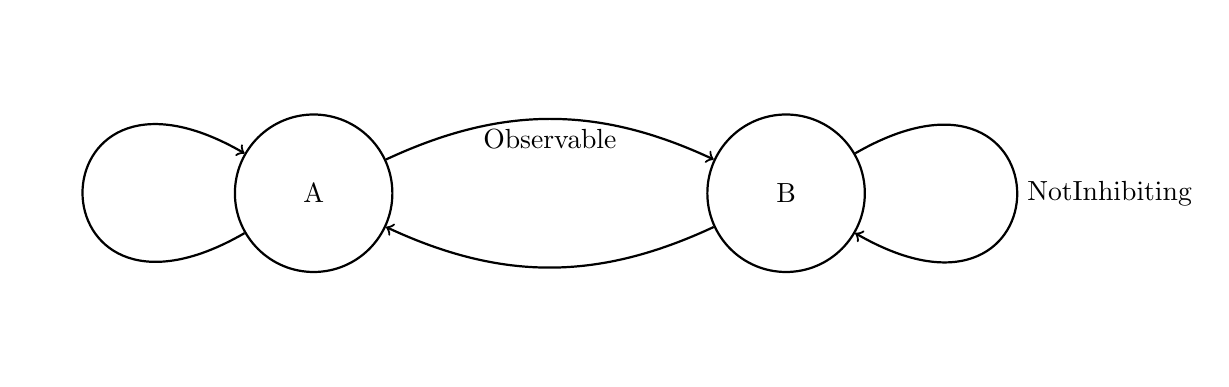
\begin{tikzpicture}
\node[draw, circle, thick, minimum size=20mm] (A) at (0,0) {A};
\node[draw, circle, thick, minimum size=20mm] (Y) at (6,0) {B};
\draw[->, thick] (A) to [in=150,out=210,loop] (A);
\draw[->, thick] (A) to [bend left=25] node[below] {Observable} (Y);
\draw[->, thick] (Y) to [bend left=25] (A);
\draw[->, thick] (Y) to [in=330,out=30,loop] node[right] {NotInhibiting} (Y);
\end{tikzpicture}
\caption{Simple example network with two components.}
\label{ExampNet}
\end{figure}

Components of such a network are usually well-know, conversely to their regulatory effects that are hard to obtain from biological measurements~\cite{Hecker09}. The Parsybone is designed to solve the task of determining those effects or at least to narrow the set of posibilities thus helping with further analysis. Possible regulatory effects of a component are given by the so-called \emph{logical parameters}. Each component has usually several logical parameters that specify towards which activity level the component inclines based on the current activity levels of its regulators e.g. a self-regulating component can stop its production when a certain concentration level is reached.

The user is required to specify the model as a set of components and their interactions. Having such a model, the Parsybone generates all possibile combinations of logical parameters for the model, creating a set of \emph{parametrizations}. This set is usually called \emph{parametrization space} and it can be viewed as a set of all behavioural possibilities for the model. As a second input, the Parsybone takes a specification of some behaviour the model must be able to reproduce. Parametrizations that do not allow such a behaviour are then removed from the set of possibilities.

Apart from basic boolean properties we also allow the model to be created using multiple extensions:
\begin{itemize}
\item Multi-valued components, allowing to change the effect of only a subset of its regulatory effects at a time.
\item Edge labels, bounding possible effects of the regulations.
\item Partial parametrizations, allowing to reduce the parametrization space before the analysis itself.
\item Basal values, specifying general case behaviour of components.
\end{itemize}

These extension allow for more precise model description than the basic boolean network formalism as presented above, but their explanation is beyond scope of this section. In case of furter interest please refer to~\cite{TechReport}.

\section{Modeling}
\label{sec:modeling}
 Models are described using an internal modeling language, based on the XML syntax~\cite{XML}, called \emph{PMF} (Parsybone model file). The model is provided within a single PMF file that holds specification of the regulatory network. 
 
For description of desired properties of the dynamical system a second file type, also based on the XML, is used. Predictably the name of the format is PPF (Parsybone property file).

Both the files must abide by the general XML rules and be provided as runtime arguments with their suffixes corresponding to their data type, i.e. with the \emph{.pmf} and \emph{.ppf} suffixes.

\subsection{Model example}
Every model must be enclosed within a pair \texttt{NETWORK} tag. A detailed description of the modeling language is provided later in this section, here we present, as an example, a model file for the network depicted in the \emph{introductory pdf}. 

This example model has a quite non-uniform syntax, which has been chosen on purpose to present different possibilities of model description.
\begin{alltt}
\input{model.pmf}
\end{alltt}
As can be seen, the model is a structure with two species, both regulated by itself and each other. For the component $B$, the possible parametrizations space is reduced by requirements that the regulation from $A$ must be observable and that the effect of its self-regulation must be positive, if any. Also, the logical parameter of self-regulation of the component $B$ must always be 1. As a result, the parametrization space is reduced to four possibilities.

\subsection{Model property}
The main purpose of the tool is picking parametrizations that satisfy some property. The description of this property can be given in one of two possible ways - either as B\"uchi automaton or as a time series. A time series is merely a B\"uchi automaton specialization, but as will be explained later the Parsybone is optimized for its usage and provides additional features if the time series is employed. To demonstrate the difference between the two, we present a single property described using each formalism. 

This property assures that the model depicted in the complementary \emph{introductory pdf} is able to reproduce a time series composed of the following three measurements:
\begin{enumerate}
\item $A=0$
\item $A \Leftrightarrow B$
\item $A=1 \wedge B=0$
\end{enumerate}
Only two out of four parametrizations allow for reproduction of this time series. To obtain them, we can describe the time series either using the B\"uchi automaton:
\begin{alltt}
\input{automaton.ppf}
\end{alltt}
Or using the time series directly:
\begin{alltt}
\input{series.ppf}
\end{alltt}
As can be seen, the second method makes the model quite shorter and should be used for description of time series.

\subsection{Regulatory network description}
\begin{mitem}
	\item \texttt{NETWORK}
	\begin{mitem}
		\item Occurrence: single, mandatory.
		\item Type: pair.
		\item Parent: none, is a root node.
		\item Description: encloses the definition of a regulatory network.
		\item Attributes: none.
	\end{mitem}
\end{mitem}

\begin{mitem}
	\item \texttt{CONSTRAINT}
	\begin{mitem}
		\item Occurrence: multiple, optional.
		\item Type: solo.
		\item Parent: NETWORK.
		\item Description: specifies additional static constraint on the parametrization space.
		\item Attributes: none.
		\begin{menum}
			\item \textit{type} 
			\begin{mitem}
				\item Occurrence: mandatory.
				\item Value: bound\_loop.
				\item Description: a nature of the constraint, for details see Section~\ref{StaticConstraints}.
			\end{mitem}
		\end{menum}
	\end{mitem}
\end{mitem}
	
\begin{mitem}
	\item \texttt{SPECIE}
	\begin{mitem}
		\item Occurrence: multiple, mandatory.
		\item Type: pair.
		\item Parent: NETWORK.
		\item Description: defines a single specie.
		\item Attributes:	
		\begin{menum}
			\item \textit{name} 
			\begin{mitem}
				\item Occurrence: optional.
				\item Value: a string containing only digits, letter and underscore.
				\item Description: name of the specie under which it will be further addressed.
			\end{mitem}
%			\item \textit{undef} 
%			\begin{mitem}
%				\item Occurrence: optional.
%				\item Value: basal/param/error.
%				\item Default: param.
%				\item Description: tells the system how it should handle values of regulatory contexts that are not specified. Basal means using a basal value, param means using all possible values and error causes error in case there are unspecified parameters.
%			\end{mitem}
			\item \textit{max} 
			\begin{mitem}
				\item Occurrence: optional.
				\item Value: natural number.
				\item Default: 1.
				\item Description: maximal activation level this specie can occur in.
			\end{mitem}
%			\item \textit{basal} 
%			\begin{mitem}
%				\item Occurrence: optional.
%				\item Value: positive integer.
%				\item Default: 0.
%				\item Description: basal activation level of this specie - the value towards which the specie tends if not specified otherwise.
%			\end{mitem}
		\end{menum}
	\end{mitem}
\end{mitem}

\begin{mitem}
	\item \texttt{REGUL}
	\begin{mitem}
		\item Occurrence: multiple, mandatory.
		\item Type: solo.
		\item Parent: SPECIE.
		\item Description: defines a single incoming regulation of the parent specie.
		\item Attributes:	
		\begin{menum}
			\item \textit{source} 
			\begin{mitem}
				\item Occurrence: mandatory.
				\item Value: name or the ordinal number of a specie.
				\item Description: name of the specie that regulates this one.
			\end{mitem}
			\item \textit{threshold} 
			\begin{mitem}
				\item Occurrence: optional.
				\item Value: natural number.
				\item Default: 1.
				\item Description: lowest activation level of the source specie that activates the regulation.
			\end{mitem}
			\item \textit{label} 
			\begin{mitem}
				\item Occurrence: optional.
				\item Value: a string, see Sec.~\ref{EdgeLabel}.
				\item Default: Free.
				\item Description: describes nature of the regulation.
			\end{mitem}
		\end{menum}
	\end{mitem}
\end{mitem}
		
\begin{mitem}
	\item \texttt{CONSTR}
	\begin{mitem}
		\item Occurrence: multiple.
		\item Type: solo.
		\item Parent: SPECIE.
		\item Description: defines integral constraints on parameters.
		\item Attributes:	
		\begin{menum}
			\item \textit{expr} 
			\begin{mitem}
				\item Occurrence: mandatory.
				\item Value: logical formula (see Section~\ref{FormulaConstruction}), variables are logical parameters.
				\item Description: defines constraints that has to be satisfied by the incoming regulations.
			\end{mitem}
		\end{menum}
	\end{mitem}
\end{mitem}
	
\subsection{B\"uchi automaton description}		
\begin{mitem}
	\item \texttt{AUTOMATON}
	\begin{mitem}
		\item Occurrence: single, present if and only if there is no sibling SERIES tag.
		\item Type: pair.
		\item Parent: none, is a root node.
		\item Description: encloses the decription of a B\"uchi automaton.
		\item Attributes: none.
	\end{mitem}
\end{mitem}		

\begin{mitem}
	\item \texttt{STATE}
	\begin{mitem}
		\item Occurrence: multiple, mandatory.
		\item Type: solo.
		\item Parent: AUTOMATON.
		\item Description: defines a single state of the automaton. The first state in the description is also considered to be the initial state of the automaton.
		\item Attributes: none.
	\end{mitem}
		\begin{menum}
			\item \textit{name} 
			\begin{mitem}
				\item Occurrence: optional.
				\item Value: string containing letters and numbers.
				\item Default: ordinal number of the tag, counting from zero.
				\item Description: name of the specie under which it will be further addressed. System also uses its ordinal number (so the first state can be addressed using the name \emph{0}).
			\end{mitem}
			\item \textit{final} 
			\begin{mitem}
				\item Occurrence: optional.
				\item Value: Boolean.
				\item Default: 0.
				\item Description: specifies if the state is final (1) or not (0).
			\end{mitem}
		\end{menum}
\end{mitem}		

\begin{mitem}
	\item \texttt{EDGE}
	\begin{mitem}
		\item Occurrence: multiple, mandatory.
		\item Type: solo.
		\item Parent: STATE.
		\item Description: defines an edge leading from the parent state.
		\item Attributes: 
		\begin{menum}
			\item \textit{target} 
			\begin{mitem}
				\item Occurrence: mandatory.
				\item Value: name or the ordinal number of the target state.
			\end{mitem}
			\item \textit{values} 
			\begin{mitem}
				\item Occurrence: mandatory.
				\item Value: logical formula (see Section~\ref{FormulaConstruction}), variables are atomic propositions.
				\item Description: conditions that must be met for the edge to be transitive.
			\end{mitem}
			\item \textit{stable} 
			\begin{mitem}
				\item Occurrence: optional.
				\item Value: Boolean.
				\item Default: 0.
				\item Description: If set to (1), the transition satisfying the edge must be a loop.
			\end{mitem}
			\item \textit{transient} 
			\begin{mitem}
				\item Occurrence: optional.
				\item Value: Boolean.
				\item Default: 0.
				\item Description: If set to (1), the transition satisfying the edge must be between different states.
			\end{mitem}
		\end{menum}
	\end{mitem}			
\end{mitem}		

\subsection{Time series description}
\begin{mitem}
	\item \texttt{SERIES}
	\begin{mitem}
		\item Occurrence: single,  present if and only if there is no sibling AUTOMATON tag.
		\item Type: pair.
		\item Parent: MODEL.
		\item Description: encloses definition of a time series.
		\item Attributes: none.
	\end{mitem}
\end{mitem}				
	
\begin{mitem}
	\item \texttt{EXPR}
	\begin{mitem}
		\item Occurrence: multiple, mandatory.
		\item Type: solo.
		\item Parent: SERIES.
		\item Description: a single measurement in the time series.
		\item Attributes:	
		\begin{menum}
			\item \textit{values} 
			\begin{mitem}
				\item Occurrence: mandatory.
				\item Value: logical formula (see Section~\ref{FormulaConstruction}), variables of the formula must be atomic propositions.
				\item Description: conditions that must be met for the measurement to be reproduced.
			\end{mitem}
						\item \textit{stable} 
			\begin{mitem}
				\item Occurrence: optional.
				\item Value: Boolean.
				\item Default: 0.
				\item Description: If set to (1), the transition satisfying the edge must be a loop.
			\end{mitem}
			\item \textit{transient} 
			\begin{mitem}
				\item Occurrence: optional.
				\item Value: Boolean.
				\item Default: 0.
				\item Description: If set to (1), the transition satisfying the edge must be between different states.
			\end{mitem}
		\end{menum}
	\end{mitem}
\end{mitem}	

\subsection{Edge label}
\label{EdgeLabel}
There are two basic labels:
\begin{itemize}
\item [+]	Meaning that the there must be a regulation whose parameter value increases if we add this regulator.
\item [-]	Has the opposite meaning.
\end{itemize}
One can compose these labels using a logical formula over $+$ and $-$ or use one of the following predefined descriptions:
\begin{itemize}
\item Activating: $+$
\item ActivatingOnly: $(+ \wedge \neg -)$
\item Inhibiting: $-$
\item InhibitingOnly: $(- \wedge \neg +)$
\item NotActivating: $\neg +$
\item NotInhibiting: $\neg -$
\item Observable: $(+ \vee -)$
\item NotObservable: $(\neg + \wedge \neg -)$
\item Free: $true$

\end{itemize}

\subsection{Static constraints}
\label{StaticConstraints}
Constraints that globally restrict the parametrization space based on certain assumptions.
\subsubsection*{bound\_loop}
This constraint serves purely to optimization of multi-valued models and should be always used, unless there is a reason not to.

In multi-valued models, a scenario where multiple different parameters spawn the same structure may occur, simply because the values lay outside the activity levels for the respective context. This constraint leaves only a single representative of this behavior.
%\subsubsection*{force\_extremes}
%This constraint simply assigns an exact target value in two cases:
%\begin{itemize}
%\item $0$ is assigned for the case when all positive regulators are absent and all negative are present.
% \item $max$ is assigned for the case when all negative regulators are absent and all positive are present.
%\end{itemize}
%For this property, an unambiguous edge constraint must be assigned - Observable, NotObservable and Free edge constraints will cause the force\_extremes switch to have not effect for the regulated component.

\subsection{Formula construction}
\label{FormulaConstruction}
A formula is constructed using the following set of recursive rules:
\begin{enumerate}
\item Depending on use, any atomic proposition or any kinetic parameter are formulae,
\item $tt$ and $ff$ are formulae representing true or false respectively,
\item if $A$ is a formula, then $\neg A$ a formula,
\item if $A,B$ are formulae, then $(A|B)$ and $(A\&B)$ are formulae representing logical disjunction and conjunction respectively,
\item nothing else is a formula.
\end{enumerate}

\subsubsection*{Atomic proposition}
An atomic proposition is a string of the form: $specie*value$, where:
\begin{itemize}
\item $specie$ denotes the name or ordinal number of a specie,
\item $*$ denotes comparison operator from the set $\{<,>,=\}$,
\item $value$ denotes a positive integer with which the value of the specie is compared.
\end{itemize}

\subsubsection*{Kinetic parameters}
A kinetic parameter is a string of the form: $context*value$. For a component $v$ with the set of regulators $v^-$ and $T(v',v)$ the set of thresholds on multi-edge from $v'$ to $v$ the context is a string of the form:
$ v_1:t_1,\dots, v_n:t_n $, where $\{v_1,\dots,v_n\} = v^-$ and $t_i \in T(v_i,v)$.

\subsubsection*{ASCII coding}
Note that in the model file
\begin{itemize}
\item $\neg$ is denoted \texttt{!}
\item $\wedge$ is denoted \texttt{\&}
\item $\vee$ is denoted \texttt{|}
\end{itemize}

Also, this description is not compliant with the XML standard. It is not necessary for Parsybone, but to increase portability we recommend to use:
\begin{itemize}
\item \texttt{\&amp;} instead $\&$ 
\item \texttt{\&lt;} instead $<$ 
\item \texttt{\&gt;} instead $>$
\end{itemize}

\section{Understanding the results}
Parsybone computes parametrizations of the network that produce model of the property used for synthesis.

The result is a table that has the columns labeled with individual contexts in the form explained in Sec.~\ref{FormulaConstruction}. Each column then describes a single valid parametrization. There are additional columns for data captured during the model checking procedure as well. In the current version of Parsybone these are Cost, Robustness and Witness.

Interpretation of data is not a uniform activity and certainly not a simple one at that. Some tools for partial automation are in development as of now, but here are some general hints.

\subsubsection*{Parametrization count}
There are two obvious extremes - if there is no parametrization produced it means that there is no model satisfying the property - it may be that there is simply an error in the property. If not, one may try to relax the conditions:
\begin{itemize}
\item Allow uncertain edges to not have an observable effect (e.g. turning ActivatingOnly into NotInhibiting).
\item Add new edges with monotonic effect (NotInhibiting, NotActivating) where one expects possible regulatory effect.
\item Relax the behavioral requirements - either by removing values that were rather ambiguous from the expressions or shortening the time series.
\end{itemize}

If there are on the other hand there is no reduction, one gets reassured that the model is in line with the requirements, however it is not very helpful for the synthesis process. 
Apart from an obvious path of trying additional properties, one can also refer to additional metrics that create ordering on parametrizations which may or may not be relevant, dependent on the exact nature of the model.

Lastly, in the special case when the size of the parametrization space is dividable by the size of remaining set or if their GCD is quite high, there is a chance that the filtering procedure removed only functions over a specific component. Such a symmetry is likely to be caused by a reduction on functions governing single target only, allowing to observe the resulting set as a product on mutually independent reductions.

\subsubsection*{Cost}
Cost denotes the shortest path that is a witness of the property being satisfied. 
For some involved formulae this value may not make sense, however in general one is interested in the parametrizations that have low cost.
Reasoning behind this value is that each discrete step is something that consumes energy of the system and in general the lower the energy consumption the better. 
This may not be logical when the reactions are occurring on completely different time-scales, however even in such cases low cost is probably preferable purely by the virtue of simplicity.

\subsubsection*{Witness}
Parsybone can reproduce the steps on a path to accepting states. 
Note that there are usually many options for non-deterministic choice - to be able to capture the different paths in a reasonable space, we print out only transitions on these paths, meaning that the result is just a set of oriented edges.

What may be of particular interest are \emph{diamond} structures, i.e. cases where there are two states in between which there are path with all the possible orderings on the changes of values.
Such a structure suggests components of the network with correlated expression but with no mutual dependencies and may also point out possible reduction point.

\subsubsection*{Robustness}
Last value available to the user is the robustness metric which computes the probability of reaching an accepting state if a random walk of a fixed length is taken. 

The greater the value is, the more deterministic is the system in reaching accepting states. Two models with the same cost but different robustness mean that the one that has a smaller robustness has more chances to diverge from its path to the accepting states. 

In case we expect the system to be serve only one function, high robustness is welcome, however in systems like pluripotent cells, high non-determinism is more preferable.

Lastly note that our framework is inherently very non-deterministic, therefore the robustness is likely to be very low in general and decrease geometrically as the cost increases.

\bibliographystyle{abbrv}
\bibliography{Manual}



\end{document}

% LocalWords:  Parsybone CLI LTL DBM GPLv GitHub MinGW GCC ver undef parametrizations REGUL observ PARAM EXPR param filename bistability reachability
